\chapter{Конструкторская часть}

В данном разделе рассматривается процесс проектирования структуры программного обеспечения.

\section{Состав программного обеспечения}

Программное обеспечение состоит из клиент-серверного приложения.

Структура разрабатываемого проекта:

\begin{itemize}
	\item[---] сервер -- программа, обрабатывающая запросы клиентов и являющаяся посредником для передачи информации от одного клиента всем остальным;
	\item[---] клиент -- программа, которая является инициатором соединения и способная генерировать события.
\end{itemize}

\section{Функциональная модель}

На рисунках \ref{fig:idef0-a0} и \ref{fig:idef0-a1} представлена функциональная модель IDEF0 нулевого и первого уровня соответственно.

\begin{center}
	\begin{figure}[H]
		\begin{center}
			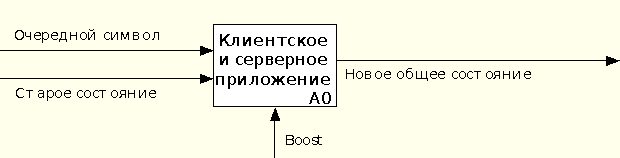
\includegraphics[scale=0.7]{img/idef0-a0.png}
		\end{center}
		\caption{\label{fig:idef0-a0} Функциональная модель IDEF0 нулевого уровня}
	\end{figure}
\end{center}

\begin{center}
	\begin{figure}[H]
		\begin{center}
			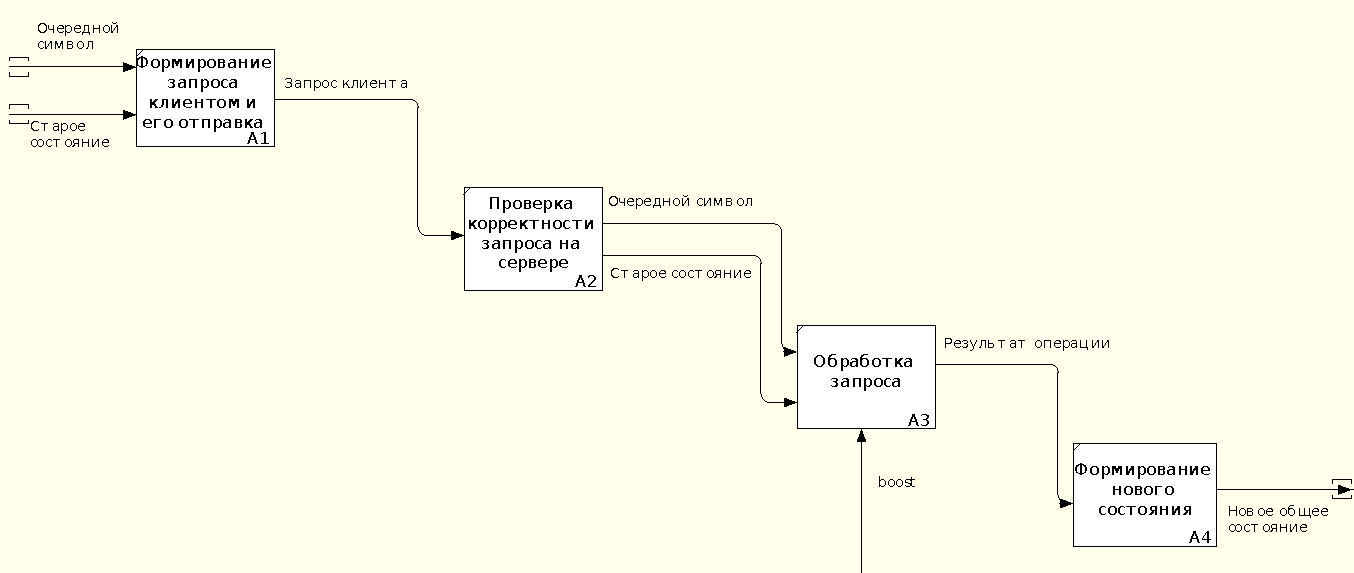
\includegraphics[scale=0.35]{img/idef0-a1.png}
		\end{center}
		\caption{\label{fig:idef0-a1} Функциональная модель IDEF0 первого уровня}
	\end{figure}
\end{center}

\section{Сценарий использования}

На рисунке \ref{fig:use-case} представлены действия доступные клиенту.

\begin{center}
	\begin{figure}[H]
		\begin{center}
			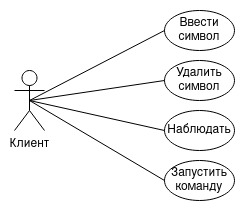
\includegraphics[scale=1]{img/usecase.jpg}
		\end{center}
		\caption{\label{fig:use-case} Use-case диаграмма}
	\end{figure}
\end{center}

\section{Проектирование протокола прикладного уровня}

Передаваемый пакет имеет следующую структуру: \texttt{пакет = (размер, сообщение)}, где \texttt{сообщение = (тип, данные)}. В свою очередь, тип может быть равен значению \texttt{getAll} либо \texttt{addChar}. 

\begin{itemize}
	\item тип запроса \texttt{getAll} сообщает серверу о необходимости вернуть клиенту изменяемое информацию о состоянии системы. Поле данных в отправляемом клиентом сообщении не заполняется;
	\item тип запроса \texttt{addChar} говорит о необходимости добавить передаваемый символ на экран и сообщить о добавлении этого символа всем подключенным клиентам. В таком случае поле данных содержат добавляемый символ и его позицию на экране;
	\item тип запроса \texttt{diff} - отправляется только от сервера клиенту и показывает, какие новые строки добавляются в неизменяемое состояние после выполнения команды. Получая этот тип, клиент также очищает текущее состояние.
\end{itemize}

Если клиент хочет добавить символ, он отправляет эту информацию серверу (запрос с типом \texttt{addChar}), сервер проверяет такой запрос на валидность, добавляет символ и сообщает всем подключенным к нему клиентам -- то есть передает новое состояние системы. Сервер может передавать клиентам лишь состояние системы.

Коды ошибок не предусмотрены -- в случае какой-либо ошибки клиент об этом узнать по средствам протокола не может. В случае невалидного запроса соединение с клиентом разрывается.

\section*{Вывод}

В данном разделе был спроектирована структура разрабатываемого программного обеспечения.

